\chapter{Modelling}

Extinction correction given by

\begin{equation}
f_{obs}(\lambda)=f_{int}(\lambda)10^{-0.4A_{\lambda}}
\end{equation}

Where $A_{\lambda}=0.213$ in the I filter around $8000 \textrm{\AA}$

\begin{figure}[H]
\centering
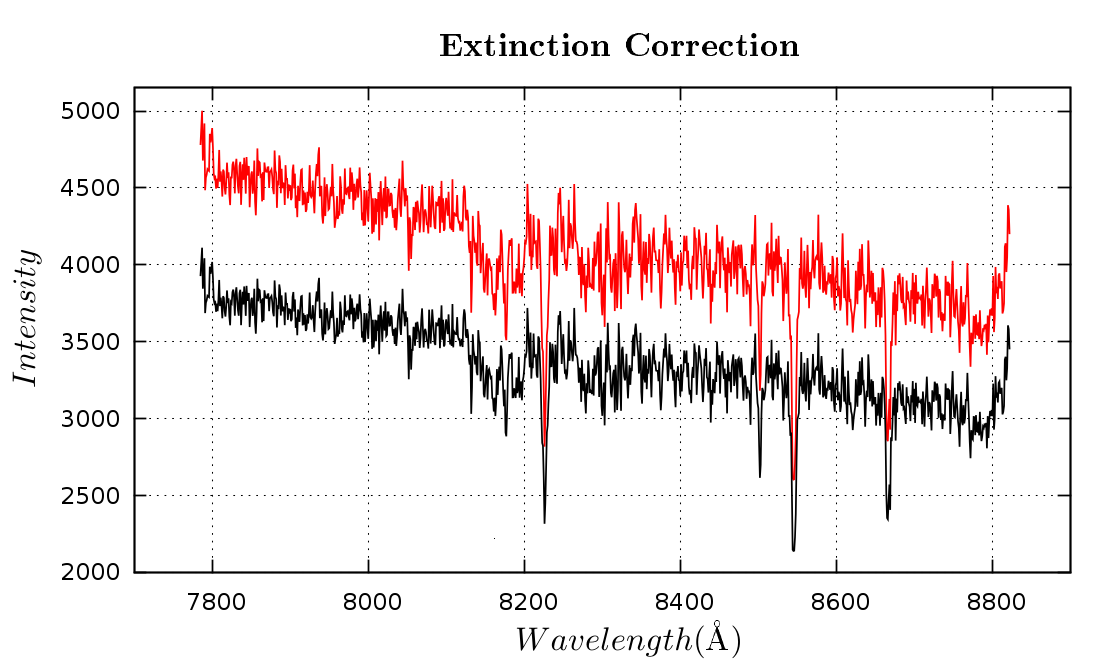
\includegraphics[width=10cm]{images/extinction.png}
\caption[Extinction Correction]{This figure shows an integrated spectrum of the central region of Omega Centauri before and after the extinction correction is applied. The black line has the original flux values and the black line has the corrected flux, that is, the flux that would be observed if there wasn't any interstellar medium that obscures the light coming from the object.}
\end{figure}

We have to multiply by a factor of 1.216746 for the flux calibration to be made.

Starlight does the stellar population synthesis 

$Mcor_tot = 3.29446 \times 10^{7}$

Yields a stellar mass of $M_{*}=243.462M_{\odot}$
